\chapter{Características y limitaciones de Azure}
\section{Características}
Las características o servicios ofrecidos por Azure son los siguientes:
\begin{figure}[h]
	\centering
	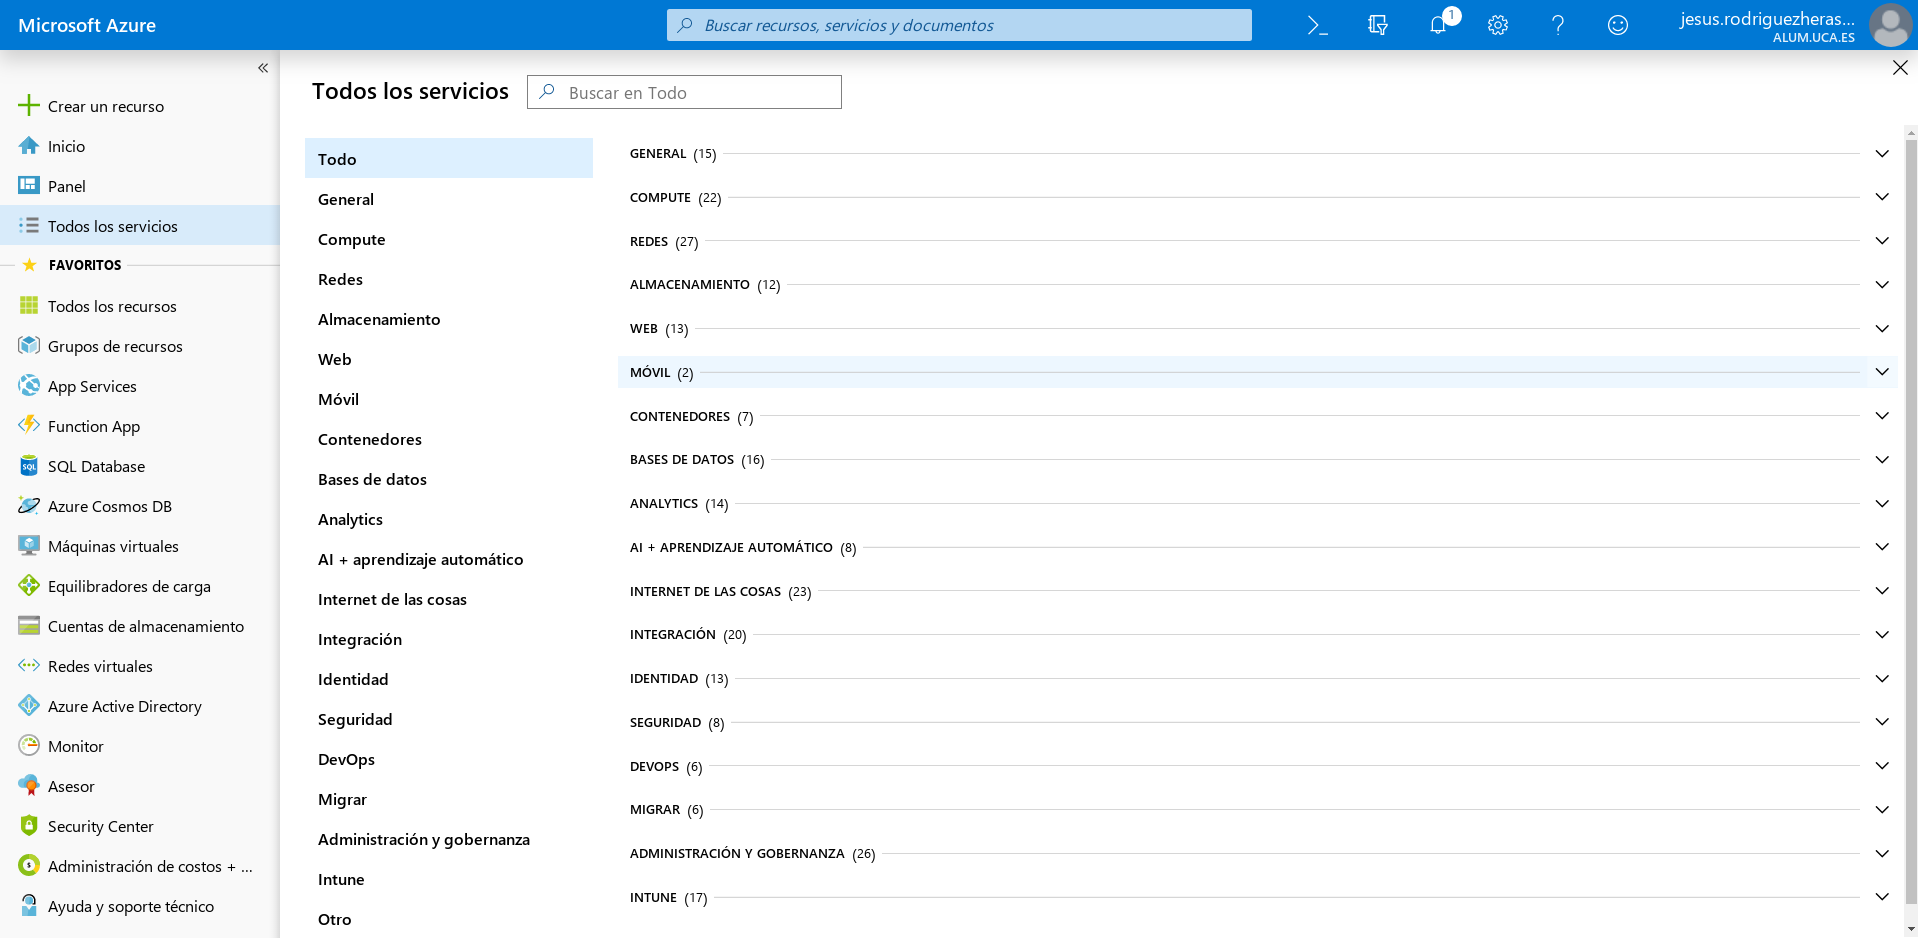
\includegraphics[scale=0.26]{ImagenesAzure/Servicios.png}
	\caption{Servicios ofrecidos por Azure.}
	\label{Servicios ofrecidos por Azure}
\end{figure}

Las características generales de Azure son las siguientes:
\begin{itemize}
	\item \textbf{Autoservicio bajo demanda:} Los usuarios pueden proveerse de cómputo en la nube sin requerir interacción humana o con el mismo proveedor.
	\item \textbf{Acceso ubicuo a la red:} Todo lo qeu podamos necesitar se encuentra en la red y accesible desde la red. Disponible desde cualquier dispositivo por medio de estándares como HTML o el protocolo HTTP.
	\item \textbf{Agrupación de recursos independientemente de la posición geográfica:} Los recursos del proveedor se encuentran geográficamente agrupados para servir a múltiples consumidores de manera distribuida y bajo demanda.
	\item \textbf{Elasticidad rápida:} Las funcionalidades se proporcionan de manera muy rápida, incluso puede ser configurable para que crezca dependiendo del ambiente actual.
	\item \textbf{Servicio medido:} El uso de todos los recursos se puede monitorizar, lo que proporciona transparencia tanto al que expone los servicios (el proveedor) como a los que acceden a ellos (los consumidores).
	\item \textbf{Pago por uso:} El costo de los servicios expuestos se puede modelar con la siguiente expresión:
	\begin{center}
		$(CaracterísticasDelServicio) * (TiempoDeActividad) = CostoTotal$
	\end{center}
\end{itemize}

Cabe destacar, y, como se ve en la figura \ref{Servicios ofrecidos por Azure} que en Azure sí contamos con servicios relacionados con Inteligencia Artificial y aprendizaje automático (Machine Learning).

\section{Limitaciones}
Dentro de la capa de estudiantes\footnote{La que hemos podido probar gracias al acuerdo de la UCA con Microsoft.} tenemos las siguientes \href{https://azure.microsoft.com/es-es/free/free-account-students-faq/}{limitaciones}, de las cuales, las más destacables son (entre muchas otras):
\begin{itemize}
	\item 750 horas de máquinas virtuales B1S\footnote{Características de las máquinas B1S: 1vCPU, 1GiB de RAM y 4GiB de almacenamiento.} tanto para Linux como para Windows.
	\item 128GB de Managed Disks\footnote{Ofrece la seguridad, disponibilidad, escalabilidad y durabilidad de HDD/SSD que se necesite para todas las cargas de trabajo, desde cargas de trabajo críticas hasta escenarios de prueba.} como combinación de dos discos de almacenamiento SSD de 64GB, además de 1GB en operaciones instantáneas y 2 millones de operaciones de E/S.
	\item 250GB de una instancia S0\footnote{Instancia de bases de datos gestionada por Azure SQL.} estándar de bases de datos SQL con 10 unidades de transacción de bases de datos.
	\item 1500 horas de IP dinámica para máquinas virtuales B1S.
\end{itemize}